\chapter{$\delta$-constraints and intensity in instrument design}
\label{chapter:constraints}
\label{c4:constraints}
Two key parameters in SEMSANS instrument design are the accessible $\delta$-range and the intensity at the detector. The first determines the range of samples that can be measured and the second the amount of signal per unit time, which determines how well you can measure in given time or similarly the measurement time needed for a required measurement quality. In this chapter, building on the analysis presented in Chapter \ref{c3}, a system of constraints will be presented that together limit the accessible $\delta$ range for each of the designs listed in Table \ref{tab:design-variants}. After discussing the $\delta$-ranges, a coarse estimate for the intensity at the detector for the two source options will be presented. Lastly, the effect of intensity loss due to SANS scattering is discussed by using a very primitive model for scattering based on the sample form factor $P(Q)$, the goal being to understand the lower $\delta$-limit of the presented instruments better.
\section{Constraints}
\label{c4.1}
Three main sources of limitations can be recognized. Firstly, the effective detector height $h_e$ and pixel size $p$ as well as the distance from detector to sample $L_s$ will limit which modulation frequencies can be sampled as well as the accessible $Q$-range, limiting $\delta$ in various ways.
Secondly, the mean wavelength $\lambda_0$ as well as the monochromator quality $\frac{d\lambda}{\lambda_0}$ (and corresponding wavelength $\sigma$) shape the modulation envelope and determine how quickly it will become too narrow as $\alpha$ increases due to increasing field strengths, with $\lambda_0$ also playing a role in all other bounds. Lastly, the basic characteristics of precession devices as well as their positions relative to the detector limit the range of $\alpha$ and how strong the precession gradient is along the $y$-axis. 

% Discuss sources of constraints, linking them to the theory in previous chapters. Ideally refer to equation numbers to avoid repetition and make it sound really solid. 
% Emphasize that these constraints serve as a starting point for estimating limitations for given instruments
\subsection{Detector sampling limitations}
Using detector sampling frequency $f_s = \frac{1}{p}$, the Nyquist frequency is $f_n = f_s/2$ and this an exclusive upper-limit at two samples per modulation period, corresponding to 
$$\delta_{max,n} = \frac{\lambda_0L_s}{2p}$$
This can be derived from the form of $\delta$ that is independent of $\alpha$, $\delta = \lambda_0 fL_s$. In practice, modulation visibility is reduced when approaching this frequency. One way to reduce this is to set a bound for this effect and solve it numerically as done in \cite{kusmin2017}. A simple alternative to this is to require more samples per period, for instance $5$ instead of $2$ giving
$$\delta_{max,s} = \frac{\lambda_0L_s}{5p}$$
Similarly, the requirement that at least 1 modulation period is visible on the detector restricts the frequency to a minimum of $f_{min} = \frac{1}{h_e}$, corresponding to 
$$\delta_{min,s} = \frac{\lambda_0L_s}{h_e}$$
An alternative and equivalent way of deriving this is through considering the detected $Q$-range, using $Q_{max}$ and $\theta_a$ as described in Section \ref{c3.4}. This gives 
$$Q_{max} = \frac{\pi h_s}{\lambda_0 L_s}$$
This is equivalent to $\delta_{min,s}$ as it satisfies $\delta_{min,s} Q_{max} = \pi$. It also provides an idea of the $Q$-range that reaches the detector, providing a coarse upper limit for $Q$ and accessible characteristic sample lengths. 

\subsection{Modulation envelope width}
As discussed before, the modulation can be described by a Gaussian envelope with a FWHM as given by Equation \eqref{eq:poly-base-modulation-fwhm}. Using $\delta = \lambda_0^2L_s\alpha$ and given a $FWHM_{e,min}$, this can be rewritten to a maximum $\delta$ value
$$\delta_{max,e} = \frac{\sqrt{2\ln 2}\lambda_0^2 L_s}{\pi\sigma FWHM_{e,min}}$$
In this way, the intuitive notion that the envelope should not become too narrow to measure enough signal can be translated to a concrete limit by choosing $FWHM_{e,min}$. For monochromators with a low $\Delta\lambda$ and a corresponding low $\sigma$ such as PG monochromators, this will in practice not normally be a limit but it can be when using velocity selectors. The chosen value in this work for $FWHM_{e,min}$ is $\SI{2}{\milli\meter}$, so $20$\% of the effective detector height $h_e$ and it is somewhat permissive.  

\subsection{Precession device limitations}
In terms of instrument design, the engineering of precession devices with a high $\alpha$ and optimizing their positions from the detector $L_1, L_2$ perhaps has the greatest impact on $\delta$-range. The importance of $L_1, L_2$ comes from the focussing condition, which is $B_1L_1 = -B_2L_2$ for two devices. As $\alpha\propto B_1 + B_2$ and $B_1, B_2$ are each limited by device-specific $B_{min}, B_{max}$ as given by Table \ref{tab:device-properties}, $B_1 + B_2$ is bounded by
$$(B_1 + B_2)_{min} = (\frac{L_1}{L_2} - 1)B_{min}$$
$$(B_1 + B_2)_{max} = (1 - \frac{L_2}{L_1})B_{max}$$
For the minimum value, $B_1 = B_{min}$ and for the maximum value, $B_2 = B_{max}$ with the other set accordingly. Using $\alpha = \frac{c(B_1+B_2)}{\pi\tan\theta_0}$, the following $\delta$ constraints can be derived
$$\delta_{min, f} = \lambda_0^2 L_s \frac{c(\frac{L_1}{L_2} - 1)B_{min}}{\pi\tan\theta_0}$$
$$\delta_{max, f} = \lambda_0^2 L_s \frac{c(1 - \frac{L_2}{L_1})B_{max}}{\pi\tan\theta_0}$$

\begin{table}[h!]
	\centering
	\begin{tabular}{c | c c | c c c}
		\toprule
		Label & $\delta_{\text{min,s}} ~[\unit{\nano\meter}]$ & $\delta_{\text{min,d}} ~[\unit{\nano\meter}]$ & $\delta_{\text{max,s}}~[\unit{\micro\meter}]$& $\delta_{\text{max,e}} ~[\unit{\micro\meter}]$ & $\delta_{\text{max,d}} ~[\unit{\micro\meter}]$ \\
		\midrule
		FOIL 4.321 & \textbf{77.8} & \num{76.3} & \num{14.2} & \num{34.3} & \textbf{3.82} \\
		WP 4.321 & \textbf{77.8} & \num{5.00} & \num{14.2} & \num{34.3} & \textbf{1.56} \\
		ISO 4.321 & \textbf{77.8} & \num{13.6} & \num{14.2} & \num{34.3} & \textbf{1.02} \\
		FOIL 8 & \textbf{144} & \num{135} & \num{26.2} & \textbf{6.35} & \num{6.73} \\
		WP 8 & \textbf{144} & \num{17.0} & \num{26.2} & \num{6.35} & \textbf{5.35} \\
		ISO 8 & \textbf{144} & \num{46.6} & \num{26.2} & \num{6.35} & \textbf{3.50} \\
		\bottomrule
	\end{tabular}
	\caption{Calculated $\delta$ constraints for the designs with the constraints limiting the final $\delta$-range listed in Table \ref{tab:designs-final-ranges} marked in bold for each design. Many values are identical due to most parameters such as lengths $L_1, L_2, L_s$ being the same. These are included for each design to facilitate comparison with the optimized designs presented in Chapter \ref{c5:optimization}.}
	\label{tab:designs-delta-constraints}
\end{table}
\section{Computed $\delta$ constraints and design $\delta$ ranges}
\label{c4.2}
The computed $\delta$-constraints for the designs are given in Table \ref{tab:designs-delta-constraints}. From these together, $\delta$-ranges can be calculated for each design as given in Table \ref{tab:designs-final-ranges} together with their $Q_{max}$. %These values were computed using $L_s = 1.8\unit\meter$, which is approximately the maximal $L_s$ setting available. This means that shorter $\delta_{min}$ is accessible by reducing $L_s$ but $\delta_{max}$ is the maximal spin-echo length that can be measured.
\begin{table}[h!]
	\centering
	\begin{tabular}{c | c c c c | cc}
		\toprule
		Label & $Q_{\text{max}} ~[\unit{\angstrom^{-1}}]$ & $\theta_a~[\unit{\milli\radian}]$ & $\delta_{min}~[\unit{\nano\meter}]$ & $\delta_{max}~[\unit{\micro\meter}]$ & $\delta_{min,abs}~[\unit{\nano\meter}]$ & $\delta_{max,abs}~[\unit{\micro\meter}]$ \\
		\midrule
FOIL 4.321 & \num{0.00404} & \num{2.78} & \num{77.8} & \num{3.82} & \num{14.4} & \num{3.91} \\
WP 4.321 & \num{0.00404} & \num{2.78} & \num{77.8} & \num{1.56} & \num{14.4} & \num{1.60} \\
ISO 4.321 & \num{0.00404} & \num{2.78} & \num{77.8} & \num{1.02} & \num{14.4} & \num{1.05} \\
FOIL 8 & \num{0.00218} & \num{2.78} & \num{144.} & \num{6.35} & \num{26.7} & \num{6.51} \\
WP 8 & \num{0.00218} & \num{2.78} & \num{144.} & \num{5.35} & \num{26.7} & \num{5.48} \\
ISO 8 & \num{0.00218} & \num{2.78} & \num{144.} & \num{3.50} & \num{26.7} & \num{3.59} \\
		\bottomrule
	\end{tabular}
	\caption{Key characteristics for the various designs, with $\delta_{min}, \delta_{max}$ being computed using the constraints listed in Table \ref{tab:designs-delta-constraints}. Also included are $\delta_{min,abs}, \delta_{max,abs}$ which indicate the absolute limits that can be measured using $L_s = L_{s,min} = \SI{0.333}{\meter}$ and $L_s = L_{s,max} = \SI{1.84}{\meter}$ respectively}
	\label{tab:designs-final-ranges}
\end{table}
\subsection{Discussion of design constraints}
The computed $\delta$-ranges and $Q_{max}$ give a first understanding of for what samples the designs can be used to estimate $G(\delta)$ through $G_{\text{exp}}(\delta)$. $\delta$ limits the range of $G(\delta)$'s that can be estimated and $Q_{max}$ gives an indication of how well the bounded integral will approximate the true value. It can be seen that instruments at $\lambda_0 = \SI{4.321}{\angstrom}$ have a wider $Q$-range given the same $L_s, h_e$ as was to be expected from $Q_{max} \propto 1/\lambda_0$ and correspondingly a lower $\delta_{min}$, making them better able to characterize samples of $\delta \approx \SI{100}{\nano\meter}$. For instruments with triangles and prisms, the condition that at least one modulation period must fit on the detector with effective height $h_e$ is a limiting factor, whereas for foils the devices and their positions $L_1, L_2$ limit $\delta$. Another observation that can be made is that instruments at $\lambda_0 = \SI{4.321}{\angstrom}$ with a narrower $\lambda$ spectrum are limited more strongly by the upper sampling limit due to detector pixel size $p$ whereas with a wider spectrum at $\lambda_0 = \SI{8}{\angstrom}$ the narrowing of the modulation envelope becomes a limiting factor. With exception of FOIL 8, the upper $\delta$ limit is in these instruments determined by device characteristics together with $L_1, L_2, L_s$ as well as the specific $\lambda_0$ operating point. 


\subsection{Limitations of constraint scheme}
Together, the constraints above give an impression of various factors limiting the achievable $\delta$-range for SEMSANS instruments with $2$ precession devices. It makes it possible to quickly evaluate designs such as those given and identify possibilities to improve them by making the necessary changes. There are some key limitations however, in particular related to the beam and the detector $Q$-range. As mentioned in Section \ref{c3.4} it is assumed that the beam covers an effective detector height of $h_e$ which translates to requirements for the beam width and/or divergence. The intensity across the beam is assumed to be uniform, which means that the used Gaussian modulation pattern might be too simple of a model for the modulation envelope. As for the $Q$-range, the lower limit imposed by sampling and the precession devices might be too permissive as in practice at the smallest $\delta$, $Q_{max}$ can be too low and $G_\text{exp}(\delta)$ can significantly deviate from $G(\delta)$, this will be discussed in Section \ref{c4.4}. $B$-resolution limitations and how these could influence the $\delta$-resolution were also not considered. Lastly, all computed constraints are derived from values as listed in Table \ref{tab:device-properties} and elsewhere meaning that if say improved precession devices are available with greater $B_{max}$ or different $\theta_0$, the constraints need to be reevaluated.  
%Some factors that were not taken into account are errors in $G_\text{exp}$ for the lowest $\delta$ values where the $Q$-range might be insufficient as well as more acc


% Discuss things that are missing
%Also very important: discuss the softer constraints: why should the envelope FWHM be 3mm and not 2mm or 4mm? What determines this other than vibes. Indicate how they could be made more/less flexible		




\section{Intensity estimate}
\label{c4.3}
In this section, a coarse estimate of intensities as they can be expected using the described designs is derived. Although accurate intensity estimates are beyond the scope of this research, requiring detailed characterizations of losses in all components as well detailed information about the newly installed cold source, a highly simplified estimate assuming ideal components can be derived as follows.

The original targetted value for the full-spectrum flux at the new cold source beamline corresponding to a reactor power of $\SI{3}{\mega\watt}$ of $\SI{1e9}{\centi\meter^{-2}\sec^{-1}}$ \cite{OYSTER2008} is taken as a starting point. It is assumed that the intensity of the source has about half the original targetted intensity, so $\Phi_0 = \SI{5e8}{\centi\meter^{-2}\sec^{-1}}$. Given an operating point $\lambda_0$ with a matching $\sigma$ from the monochromator type, the intensity can be estimated by numerical evaluation of the integral
$$\Phi_{mc} \propto \int_0^\infty f_\lambda(\lambda)e^{-\frac{1}{2}\left(\frac{\lambda - \lambda_0}{\sigma}\right)^2}d\lambda \Phi_0= C_{mc}\Phi_0$$
The transfer of the monochromator is assumed to be a lossless Gaussian, and losses from beam divergence from beamline to monochromator are neglected.  It can easily be seen from Figure \ref{fig:source-spectrum} that the choice of $\lambda_0$ matters here, as well as the value of $\sigma$. For the used monochromators at $\lambda_0 = \SI{4.321}{\angstrom}$ and $\lambda_0 = \SI{8}{\angstrom}$ with $\Delta\lambda = \SI{0.4321}{\angstrom}$ and $\Delta\lambda = \SI{0.8}{\angstrom}$ the integral on the left evaluates to $C_{mc} = 0.00631826$ and $C_{mc} = 0.07346646$. Assuming an ideal polariser and an ideal analyser, the average loss of intensity for $\pm x$ analyser settings due to these corresponds to a factor $1/4$. To account for losses due to beam divergence, consider the beam divergence to be a small angle $\psi_0$. 
For a uniform beam of radius $R_0$ coming out of the beamline with such a divergence $\phi_0$, it will have expanded to radius $R = R_0 + \psi_0 d$ in small-angle approximation. Simplifying the distribution of neutrons to be uniform over this radius after expansion, the flux at distance $d$ behind the analyser can be seen to be proportional to
$$\Phi(d) \propto \frac{\Phi_{mc}}{4}\frac{R_0^2}{(R_0 + \psi_0 d)^2} = \frac{\Phi_0}{4}C_{mc}C_{div}$$
Consider $R = \SI{0.1}{\meter}$ to be the radius of the beamline and let $\phi_0 = \SI{2}{\deg}$. Using $d = \SI{6}{\meter}$ as estimate for the distance of the sample to the beamline gives a divergence loss factor of about $C_{div} = 0.1044$.

Using this approach gives highly optimistic order of magnitude estimates of the flux at the sample for both $\lambda_0$ options: $100021 \approx \SI{1e5}{\centi\meter^{-2}\sec^{-1}}$ and $959064 \approx \SI{1e6}{\centi\meter^{-2}\sec^{-1}}$ for $\lambda_0 = \SI{4.321}{\angstrom}$ and $\lambda_0 = \SI{8}{\angstrom}$ respectively, the order of magnitude difference being due to the greater $\Delta\lambda/\lambda_0$ of the velocity selector compared to the PG crystal under the assumption of an optimal Gaussian transfer. As the detector has an area of approximately $\SI{1}{\centi\meter^2}$ and neglecting additional losses due to further divergence, this is also roughly the total intensity at the detector, at least in the absence of a sample or when using a sample that scatters only into a very small $Q$-range. Various losses due to non-ideal components etc. can be expected to reduce these estimates by perhaps another of magnitude and the relative efficiency of concrete PG and VS monochromators could cancel the estimated benefit of the VS.

\section{Sample scattering and intensity}
\label{c4.4}
Although so far the the accessible $\delta$-range and detector intensity have been discussed separately, the characteristic length of the sample measured will have a tangible effect on the measured intensity as well as the quality of $G_{exp}(\delta)$ as estimate of $G(\delta)$ limited to $Q_{max}$ for lower $\delta$ and higher $\lambda_0$. This effect was first discussed in the context of SESANS with an instrument for which $\lambda_0 = \SI{2}{\angstrom}$ and $\theta_a \approx \SI{30}{\milli\radian}$ \cite{rekveldt1996}, where it was concluded that for characteristic lengths larger than $\SI{5}{\nano\meter}$ SESANS can be used to reliably estimate $G(\delta)$. Using $L_s = \SI{1.8}{\meter}$ for the instruments considered here, $\theta_a \approx h_e / (2L_s) = \SI{2.8}{\milli\radian}$. With $\lambda_0 = \SI{4.321}{\angstrom}$ and $\lambda_0 =  \SI{8}{\angstrom}$, this estimated limit translates to about $\SI{100}{\nano\meter}$ and $\SI{200}{\nano\meter}$ respectively. This indicates that the true $\delta$-range might be more limited using current $h_e,L_s$ and the colder wavelengths. This effect is here verified using a very primitive non-randomized computational approach from which deviation from the ideal regime in which almost all scattered neutrons reach the detector \cite{rekveldt1996} can be seen. 
\begin{figure}[htbp]
	\centering
	\begin{subfigure}[b]{0.49\textwidth}
		\centering
		\includegraphics[width=\textwidth]{simplified-I-scattering-3D-plot-point-4.321}
		\caption{Scattering from point $(s_x,s_y) = (0,0)$ projected onto the detector plane.}
		\label{fig:simplified-scattering-3D:a}
	\end{subfigure}
	\hfill
	\begin{subfigure}[b]{0.49\textwidth}
		\centering
		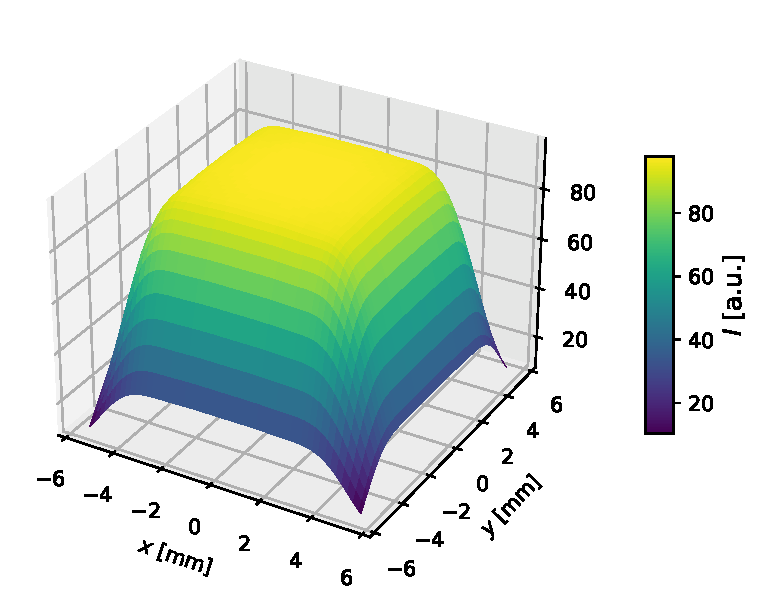
\includegraphics[width=\textwidth]{simplified-I-scattering-3D-plot-4.321}
		\caption{Scattering integrated over entire sample and normalized.}
		\label{fig:simplified-scattering-3D:b}
	\end{subfigure}
	\caption{An illustration of a simple scattering model assuming a very thin sample and single scattering of a square beam with $R= \SI{200}{\nano\meter}$, $\lambda_0 =  \SI{4.321}{\angstrom}$ and $L_s = \SI{1.8}{\meter}$. Beam divergence is neglected and a uniform profile is assumed. Figure \ref{fig:simplified-scattering-3D:a} shows the intensity contribution of a single point $(s_x,s_y) = (0,0)$ projected onto the detector. Figure \ref{fig:simplified-scattering-3D:b} shows the normalized result of integrating over the full $10\times10~\unit{\milli\meter}$ sample, giving an indication of how much of the scattered fraction of neutrons is detected and which part of the detector can be used to reliably compute $G_\text{exp}$ without resorting to Monte Carlo methods.}
	\label{fig:simplified-scattering-3D}
\end{figure}
\begin{figure}[htbp]
	\centering
	\begin{subfigure}[b]{0.49\textwidth}
		\centering
		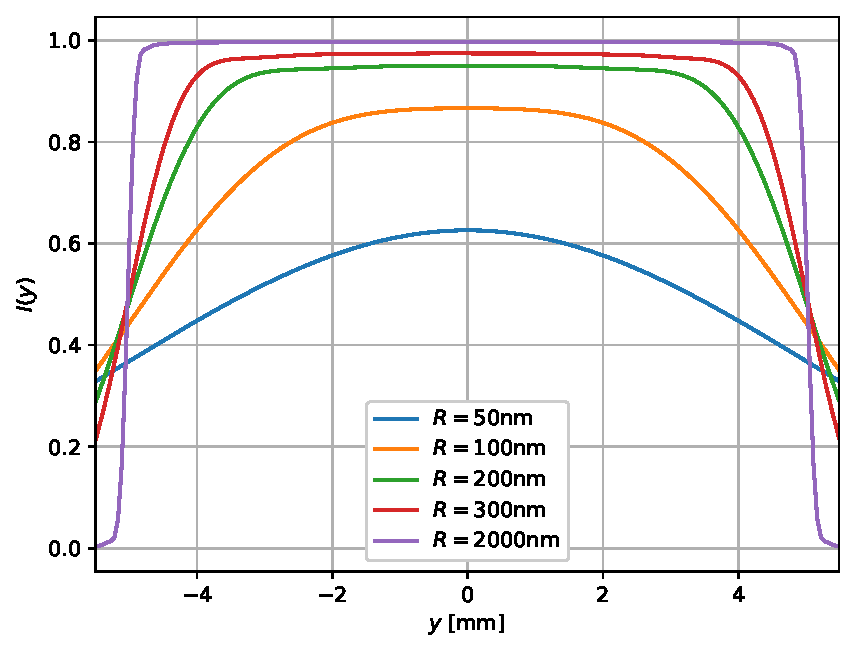
\includegraphics[width=\textwidth]{simplified-I-scattering-4.321}
		\caption{Estimated detected scattering fraction for $\lambda_0 = \SI{4.321}{\angstrom}$}
		\label{fig:simplified-scattering-4.321}
	\end{subfigure}
	\hfill
	\begin{subfigure}[b]{0.49\textwidth}
		\centering
		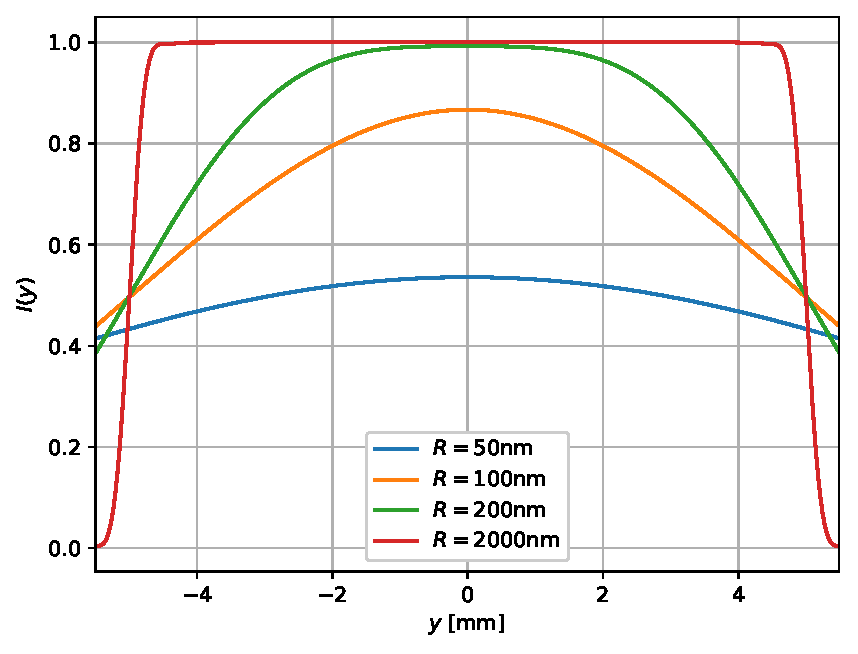
\includegraphics[width=\textwidth]{simplified-I-scattering-8.0}
		\caption{Estimated detected scattering fraction for $\lambda_0 = \SI{8}{\angstrom}$}
		\label{fig:simplified-scattering-8}
	\end{subfigure}
	\caption{A comparison of the estimated fraction of scattered neutrons that is detected at each point on the detector with $L_s = \SI{1.8}{\meter}$ for $\lambda_0 = \SI{4.321}{\angstrom}$ and $\lambda_0 = \SI{8}{\angstrom}$ and different radii $R$. Curves are calculated by first computing a 2D intensity pattern as illustrated in Figure \ref{fig:simplified-scattering-3D:b}, after which the pattern is integrated over $x$ and normalized.} 
	\label{fig:simplified-scattering}
\end{figure}
\subsection{Non-randomized single-scattering model}
A very thin, dilute sample of solid spheres has $d\sigma/d\Omega \propto P(Q)$ at each point in the sample $(s_x, s_y)$, neglecting effects like multiple scattering. The form factor $P(Q)$ of a solid sphere is given by Equation \eqref{eq:sample-form-factor}. Assuming a uniform square non-divergent beam where each neutrons scatters exactly once of the sample over an area of $10\times10~\unit{\milli\meter}$, the corresponding detector intensity shape can be estimated by considering each point in the sample a source of scattering with intensity proportional to $P(Q)$, which can be translated to a point $(x,y)$ on the detector using trigonometry. The corresponding detector intensity shapes are found by integrating the scattering of many such points sources, a process shown in Figure \ref{fig:simplified-scattering-3D}. 


The intensity was integrated over the $x$-axis to give a single value for each point $y$, which is also what happens at a real linear 1D detector as considered in this work. Such integrated intensity profiles for different wavelengths and radii are shown in Figure \ref{fig:simplified-scattering}. It can be seen that the respective estimated limits of $\SI{100}{\nano\meter}$ and $\SI{200}{\nano\meter}$ describe the simplified scattering behaviour quite well, with these particle radii being approximately the limit where the middle of the detector picks up almost full intensity uniformly for a certain central width. Integrating these curves could provide another sample-dependent correction factor to complement the estimate given in Section \ref{c4.3} but Figure \ref{fig:simplified-scattering} also gives an idea at which radii error in $G_\text{exp}(\delta)$ becomes significant. This is an effect which can be corrected for \cite{kusmin2017}. It should be noted that Figure \ref{fig:simplified-scattering} only models the intensity of scattered neutrons and ignores multiple scattering. The scattering power $\tau = \sigma t$ of the sample as well as factors like beam divergence and uniformity will shape the true intensity shapes and $Q$-range of scattered neutrons.  Monte Carlo methods are more suitable for such more accurate calculations and this is the subject of Chapter \ref{c6:monte-carlo}.


\section{Design evaluation}
In this chapter, a wide range of effects limiting the $\delta$-range of designs have been discussed and computed for the design variants listed in Table \ref{tab:design-variants} with their various precession devices and $\lambda_0$-monochromator pairings. An optimistic order of magnitude estimate of intensity was made giving $\SI{1e5}{\centi\meter^{-2}\sec^{-1}}$ and $\SI{1e6}{\centi\meter^{-2}\sec^{-1}}$ for $\lambda_0 = \SI{4.321}{\angstrom}$ and $\lambda_0 = \SI{8}{\angstrom}$ respectively, the difference being due to the idealized VS monochromator passing through a broader spectrum. The various upper and lower $\delta$-limits imposed by the detector, precession devices and $\lambda$-spectrum width $\sigma$ were computed and are given in Table \ref{tab:designs-delta-constraints}, resulting in the final $\delta$-ranges as given in Table \ref{tab:designs-final-ranges}. It was also shown that for the given acceptance angle $\theta_a \approx h_e / (2L_s) = \SI{2.8}{\milli\radian}$ at (approximately) maximal sample distance $L_s = \SI{1.8}{\meter}$, and given these values of $\lambda_0$, it might prove to be difficult to access $\delta\propto \SI{10}{\nano\meter}$. It would help to decrease $L_s$, increasing $\theta_a$ at the cost of slightly increasing the small-angle error as discussed in Section \ref{c3.5}. Simply decreasing $L_s$ would scale $\delta_{min}, \delta_{max}$ proportionately however, which in almost all cases would not improve the ability of instruments to measure the full target range of $\SI{10}{\nano\meter}$ to $\SI{5}{\micro\meter}$ at a single sample to detector distance $L_s$ considering Table \ref{tab:designs-final-ranges}. Increasing $h_e$ would also increase $\theta_a$ without scaling down the $\delta$ range but this would potentially require a new detector. Such optimizations with more free parameters like distances $L_s, L_1, L_2$ are the subject of the next chapter. As was to be expected since $\delta \propto \lambda_0^2$, the designs at $\lambda_0 = \SI{8}{\angstrom}$ have higher maximum $\delta$ as well as having a smaller $Q_{max}$. As far as the precession devices are concerned, the great range in terms of $\alpha$ seems to make foil flippers and Wollaston prisms interesting options for an eventual realization. The range of the two instruments using isosceles triangles appears to be too limited to be practical in an instrument which requires a high $\delta_{max}/\delta_{min}$. Although the designs using foil flippers appear to perform the best in the sense of the limits given in Table \ref{tab:designs-final-ranges}, it should be noted that the $\lambda$-dependence \cite{kraan2003} of the foils was not considered here.